\chapter{Development of Analytical Approach}
\todo[inline]{replace CITEME tags in Development of Analytical Approach}

\section{Comparative genomics predicts of \textit{cis}-regulatory elements in mosquitoes \cite{Sieglaff2009}}

\begin{figure}[hp]
\centering

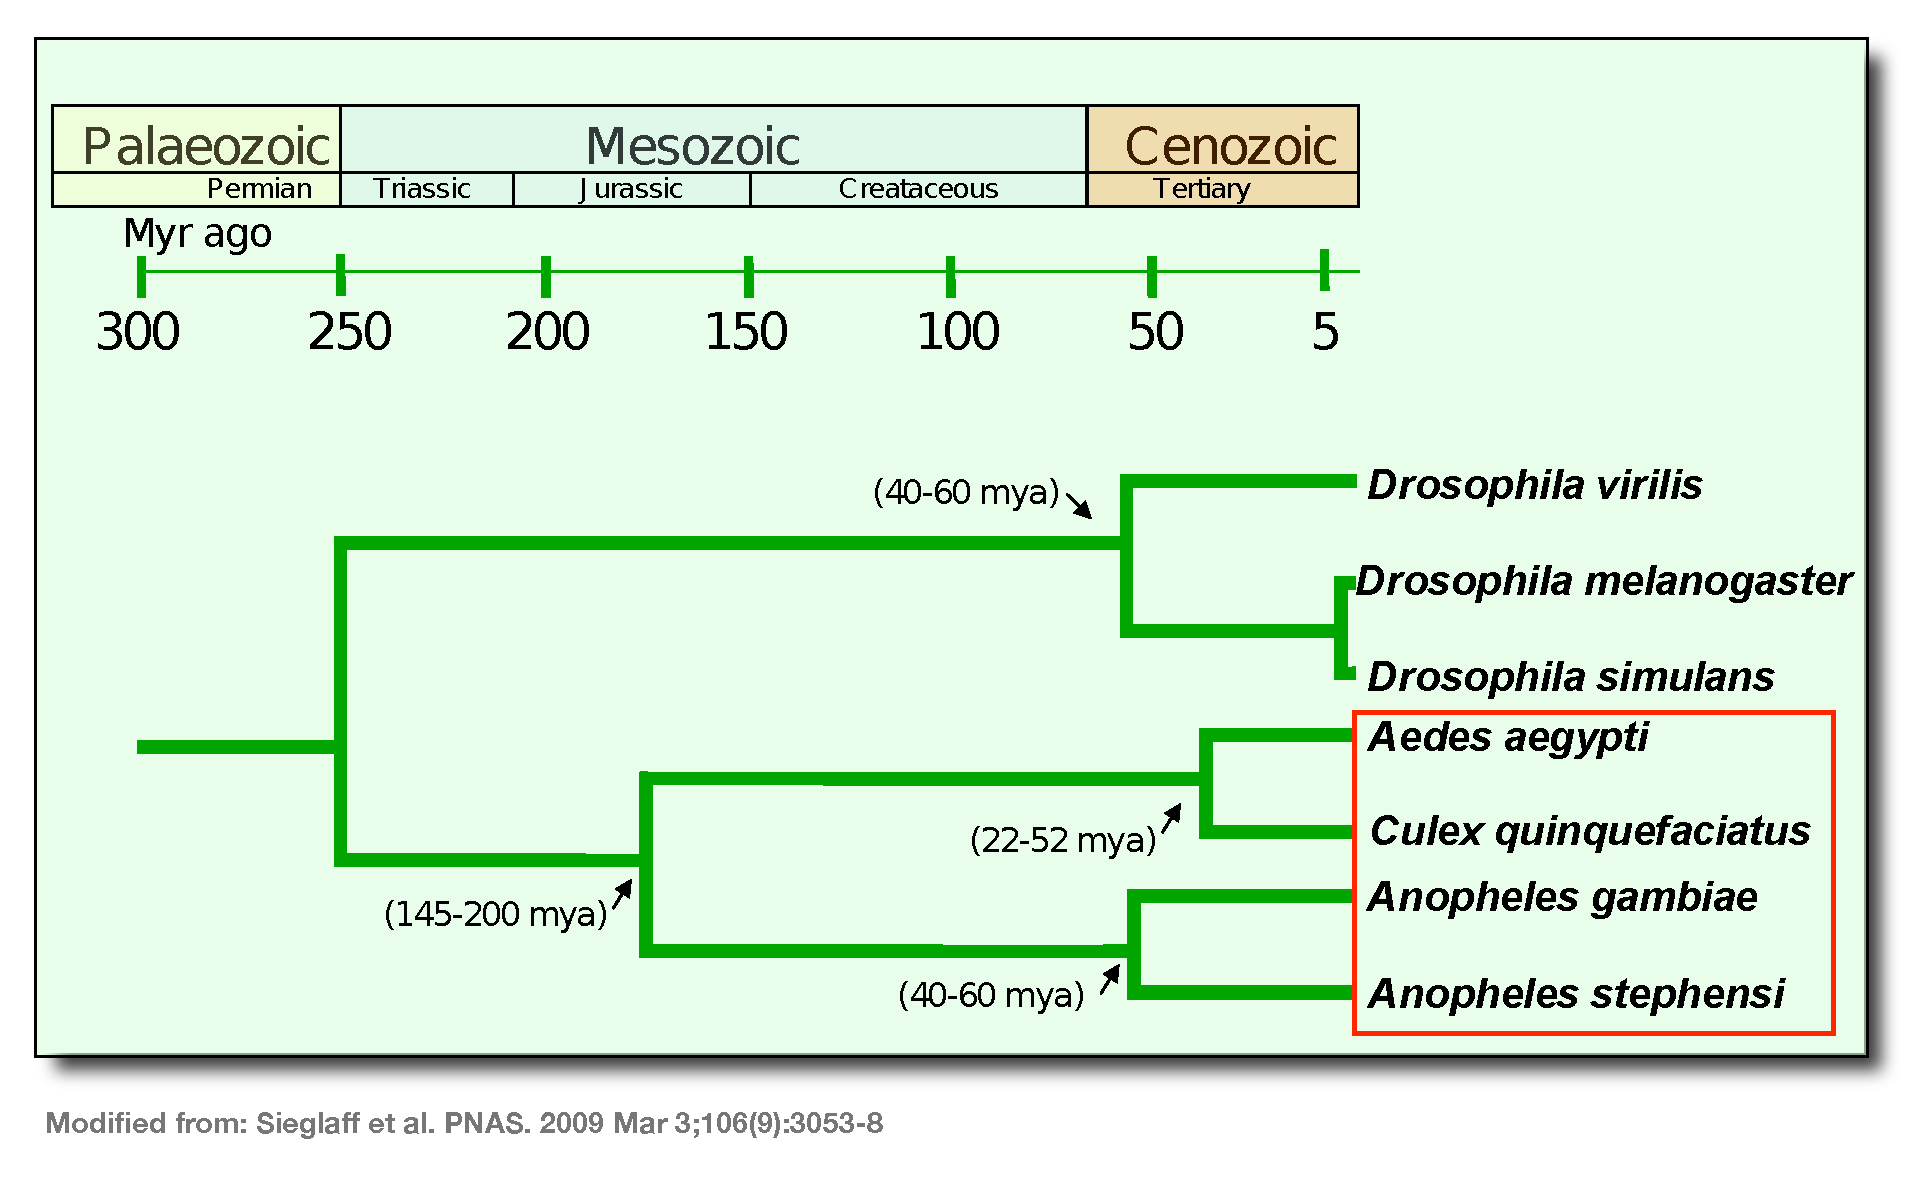
\includegraphics[width=.7\textwidth]{figures/figs/mosqPhyloTree.pdf}

\caption[Phylogenetic relationships between four vector mosquitoes]{\bsf{Phylogenetic relationships between four vector mosquitoes compared with representative \textit{Drosophila} species:} \\ \sf
\dummytext[1]

Adapted from \cite{Sieglaff2009}}
\label{fig:mosqPhyloTree}
\end{figure}

\begin{figure}[hp]

\hfil
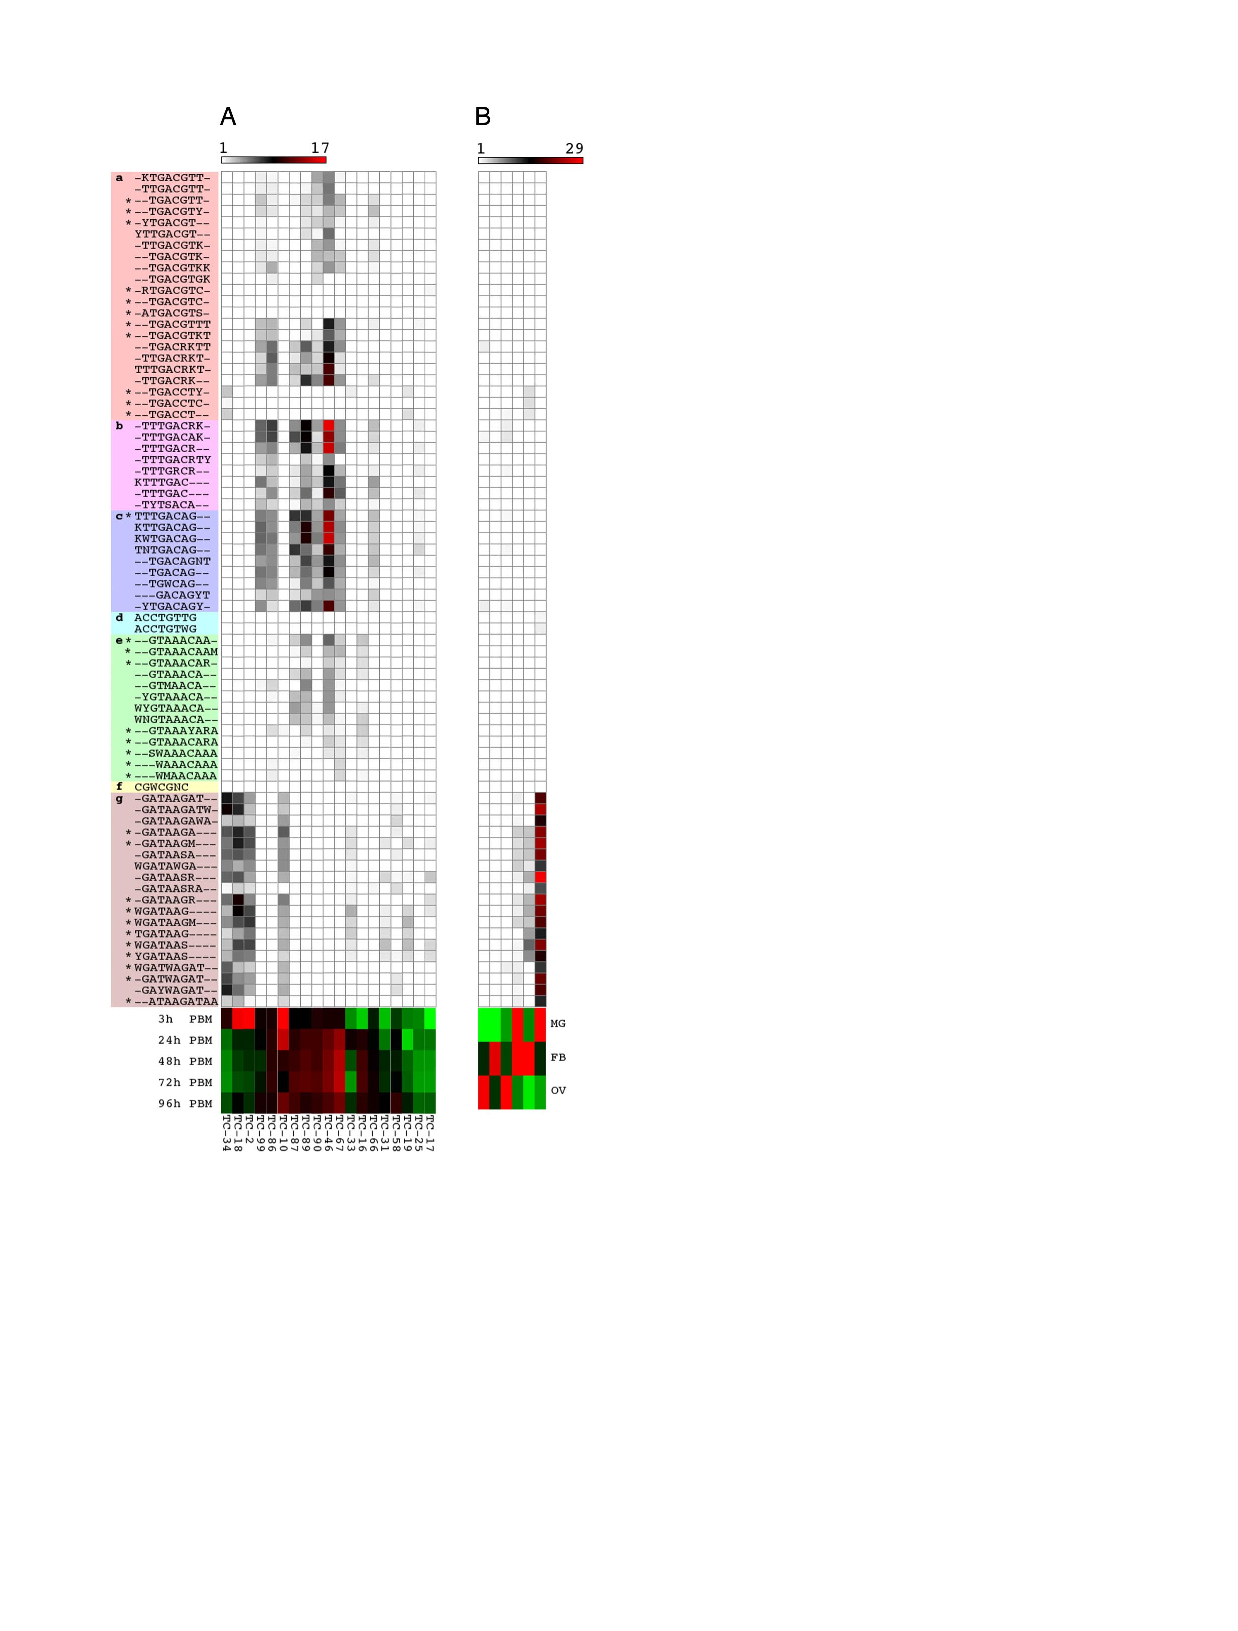
\includegraphics[scale=.95]{figures/figs/sieglaff2009_full.pdf}
\hfil
\caption[Associations of mosquito motifs with gene expression profiles in \Ag]{\bsf{Associations of mosquito motifs with gene expression profiles in \Ag:} \\ \sf
Motif enrichment within (A) 5′-end flanking regions of genes in clusters responsive to blood meal ingestion, and in (B) 5′-end flanking regions of genes in clusters enriched in selected tissues. The significance of motif enrichment is indicated by pseudocolor of -log10 (P-value) determined through hypergeometric statistics, and the median expression profile of each gene cluster is shown below each respective column. Red and green colors represent higher and lower relative mRNA accumulation, respectively. Asterisks (*) indicate a match to a previously described mosquito TFBS. Heatmaps were created with Matrix2png (\CITEME:local-58). FB, fat body; hPBM, hours post blood meal; MG, midgut; OV, ovaries; TC, time course clusters.

Adapted from \cite{Sieglaff2009}}
\label{fig:sieglaff2009_full}
\end{figure}

% [*\CITEME 3]  \cite{Nene2007}
% [*\CITEME 10] \cite{Wu2008}
% [*\CITEME 25] \cite{Kokoza2001}
% [*\CITEME 26] \cite{Cho2006}
% [*\CITEME 28] \cite{Attardo2003}
% [*\CITEME 29] \cite{Ahmed1999}
% [*\CITEME 30] \cite{Pham2005}
% [*\CITEME 32] \cite{Giannoni2001}
% [*\CITEME 33] \cite{Davidson2010}
% [*\CITEME 34] \cite{Das2007a}
% [*\CITEME 35] \cite{Hu2005}
% [*\CITEME 36] \cite{Tompa2005}
% [*\CITEME 37] \cite{Wasserman2004}
% [*\CITEME 38] \cite{Elemento2005}
% [*\CITEME 39] \cite{Stark2007}
% [*\CITEME 40] \cite{Xie2005}
% [*\CITEME 41] \cite{Dittmer2003}
% [*\CITEME 42] \cite{Meredith2006}
% [*\CITEME 43] \cite{Hernandez-Romano2008}
% [*\CITEME 44] \cite{Rai1999a}
% [*\CITEME 45] \cite{Borkent2004}
% [*\CITEME 46] \cite{Calvo2006}
% [*\CITEME 47] \cite{Adelman2007}
% [*\CITEME 48] \cite{Xu2005a}
% [*\CITEME 49] \cite{Jasinskiene2007}



The role \glspl{CRE} play in regulating gene expression during development is well-established \cite{Davidson2010}, and the development of tools for their identification is an active area of research following the publication of genome sequence and associated genome-wide expression datasets. However, the discovery \textit{in silico} of \glspl{CRE} is challenging because typically they are short, degenerate, and contained within vast amounts of intergenic genomic DNA. Despite these limitations, various computational approaches have been developed for their discovery \cite{Das2007a,Hu2005,Tompa2005,Wasserman2004}. Comparative genomics represents a powerful extension to \gls{CRE} discovery that diminishes these effects. Functional gene regulatory elements, including \glspl{CRE}, are proposed to diverge at much lower rates compared to neutral sequences because of selective pressures, and therefore may stand out from surrounding neutral DNA by virtue of their greater levels of conservation among orthologous sequences. Previous work has demonstrated the utility of this concept \cite{Elemento2005,Stark2007,Xie2005} and comparative genomics of insects has been applied successfully to map putative \glspl{CRE} in the genomes of relatively closely related \textit{Drosophila} species, [divergence times estimated ≤ 50 \gls{Mya} \cite{Stark2007} (Figure \ref{fig:mosqPhyloTree})], in which orthologous intergenic sequences are aligned more easily. The work represented here includes mosquito species with phylogenetic relationships spanning 20 to 200 \gls{Mya} with genomic comparisons complicated by large amounts of dispersed repetitive elements \cite{Nene2007}.

The \gls{MDOS} algorithm \cite{Wu2008} was designed to mitigate these problems by not requiring alignment of orthologous sequences, and incorporating features that account for the greater probability for the co-occurrence of a motif because of shared ancestry in orthologous sequences. The application of \gls{MDOS} for computational discovery of putative \glspl{CRE} shared among mosquitoes resulted in the identification of mosquito-specific or enriched motifs. These motifs demonstrate that \gls{MDOS} can identify related DNA sequences in diverged mosquitoes and may be useful in similar scenarios in which genome sequences are being analyzed for species that have no other closely related genomes available. Furthermore, the identification \textit{in silico} of GATA-factor and other \gls{TFBS} that are identical to those whose function was established experimentally \cite{Kokoza2001,Cho2006,Attardo2003,Ahmed1999,Pham2005,Giannoni2001,Dittmer2003,Meredith2006} serves as a powerful positive control for these analyses. The 5′-end regions of immune-related genes from \Ag\ and \Dm\ were screened for conserved motifs, and AT-rich domains were found to associate with \gls{NFKB} response elements \cite{Hernandez-Romano2008}. These sequences were not identified in these analyses because the restrictions on the dataset used eliminated many of the immune-related genes where one-to-one orthology may be difficult to establish. In addition, most AT-rich domains discovered in their study were ≤ 6 nucleotides in length, and these analyses only addressed those recovered with lengths of 7 to 9 nucleotides.

The 3 mosquito species included in this study require a blood meal for successful reproduction. Although this trait is not unique to this group of arthropods, acquiring the necessary nutrients for egg development from ingested blood is a specialized adaptation in insects. There is debate on when and how \gls{hematophagy} arose in mosquito evolution \cite{Rai1999a}, but it is hypothesized that the occurrence of this trait in the larger clade is \gls{monophyletic} \cite{Borkent2004,Calvo2006}. Most of the discovered mosquito motifs are associated with blood meal-regulated genes. Thus, these data support a common hematophagous ancestor for all mosquitoes, and indicate that \gls{hematophagy} acts as a selective force for conservation of \glspl{CRE}.

The functionality of some of the discovered motifs was supported further in \Ag\ and \Aa\ by their association with genes displaying enriched transcription product accumulation within tissues responsible for blood meal digestion and reproduction (Figure \ref{fig:sieglaff2009_full}). These findings bolster the conclusion that these mosquitoes share a regulatory code controlling expression levels for some genes regulated after \gls{hematophagy}. The availability of additional genome-wide studies of gene expression for all 3 mosquito species will facilitate discovery of other associations of the motifs with specific gene-regulation patterns.

This study and similar genome-wide approaches to identify putative \glspl{CRE} in mosquitoes \cite{Hernandez-Romano2008} are furthering our understanding of the mechanisms involved in gene regulation in this group of vector insects. An expanded set of putative mosquito \glspl{CRE} will allow the definition of genome-wide motif-association maps and the identification of \glspl{CRM} comprising multiple, linked \glspl{CRE} that convey specific patterns of gene expression. Experimental validation of the functionality of each discovered motif and regulatory module is necessary and will provide support for the development of mosquito synthetic promoters that deliver desired and predetermined expression patterns in transgenic mosquitoes. Promoters that direct expression of transgenes specifically to the germ cells would be useful for the development of gene-drive mechanisms for spreading a desired (pathogen-resistance) trait in a mosquito population \cite{Adelman2007}. Gene-specific knockdown or robust expression of exogenous odorant receptors or odorant binding proteins in the antenna of \gls{anthropophilic} mosquitoes could redirect their preferences toward other animals \cite{Xu2005a}. Targeted expression of antipathogen effector genes in the \glspl{midgut}, salivary glands, and \gls{hemolymph} (via fat body-specific control DNA), 3 sites of interaction of most pathogens with their insect vectors, could reduce mean intensities of infection to zero, preventing pathogen transmission and disease \cite{Jasinskiene2007}. The availability of defined synthetic mosquito promoters that direct controlled, local gene expression in response to pathogens also would be a major advance. These promoters will allow engineering of mosquitoes with increased parasite or virus resistance. These and similar envisioned applications for mosquito control and the control of mosquito-borne disease transmission will benefit greatly from a better understanding of gene regulation mechanisms in these insects.










\pagebreak

\section{RNA-seq analyses of blood-induced changes in gene expression in the mosquito vector species, \Aea\ \cite{Bonizzoni2011}}
% [-17] Brackney2010
% [-31] Fischer2008
% [-32] Pane2007
% [-33] Lawson2009
% [-50] Salazar2007
% [-54] Marelli2006
% [-55] Amenya2010
% [-56] Carlson2007
% [-57] Kriventseva2008
% [-58] Sieglaff2009
% [-60] Hubbard2002
% [-61] GENEBUILD?
% [-62] Bennet2002
% [-63] Black2002
% [-64] Terenius2008



Bonizzoni and Dunn \cite{Bonizzoni2011} provides a detailed examination of the changes in transcripts accumulation occurring at the whole-body level of \Aa\  females 5 hours \gls{PBM}. The observed changes are consistent with the beginning of an intense physiological response to a bloodmeal. The majority of immunity-related transcripts tended to accumulate at lower levels in blood fed mosquitoes. This finding supports the hypothesis that there may be a gap in immunity following a bloodmeal. Reduced expression of immune genes in blood fed mosquitoes could favor the establishment of infections, especially considering that pathogens such as dengue viruses infect the midgut epithelial cells within minutes after the contact \cite{Salazar2007}. However, changes in transcript abundance observed at the whole-body level may mask changes in accumulation occurring primarily in the midgut. Different levels of activation of immunity genes after a blood feeding may be one of the factors contributing to the variability in vector competence for dengue viruses observed in different geographic populations of \Aa\  \cite{Bennet2002,Black2002}. The quantity and quality of data generated by RNA-seq technology makes this an ideal approach for comparative analyses of the transcriptome of \Aa\ strains with different vector competence and vectorial capacity.

Our analyses of the expression profiles of sugar-fed (S) and bloodfed (B) mosquitoes allowed the identification of co-regulated genes and putative \textit{cis}-regulatory elements and modules from the \Aa\  genome. Further knowledge of the mechanisms involved in regulation of gene expression in vector species is critical to the development of control strategies whereby the vector is modified genetically to express anti-pathogen effector molecules in tissue-specific and time-regulated manners \cite{Terenius2008}. Promoter and other \textit{cis}-acting regulatory DNA fragments are needed to regulate restricted expression of selected anti-pathogen effector molecules. Moreover, we described several examples of how the RNA-seq data generated can help improve the current annotation of the \Aa\  genome.

\subsection{Transcripts found exclusively in bloodfed mosquitoes}
Forty transcripts were found only in bloodfed mosquitoes, with the highest read-counts reaching ~1000/transcript, after normalizing for different library sizes (data not shown). Functional parent attribution for these transcripts is consistent with a role in digestion and in the progression of the gonotrophic cycle. Specifically, two transcripts, Aa5G1 (AAE013712-RA) and AaSPVI (AAE010196-RA), correspond to the midgut serine proteases shown previously to be elicited by a bloodmeal in the midgut of \Aa\  females \cite{Brackney2010}. Seven other transcripts encode enzymes (i.e. decarboxylase, cathepsin b and trypsins), and two are implicated in trafficking. Transcripts AAE014815-RA and AAE005950-RB correspond to the vacuolar protein sorting 13B from yeast and the chloride channel protein 2, respectively. Ten transcripts are paralogous to the G12 gene of \Ag\ and share the Insect Allergen Repeat motif. This motif is hypothesized to be a novel, insect-specific detoxifying domain implicated in the co-evolution of herbivorous insects and their plant hosts and also has been linked to nitrile-specific detoxification \cite{Fischer2008}. Transcripts AAEL006126-RB and AAEL008921-RC are predicted orthologues of the \Cxq\ vitellogenin-A1 gene and the \Dmel\ spaghetti squash (sqh) gene, respectively. The sqh gene product encodes the regulatory light-chain of non-muscle myosin II, which is required for cytoplasmic transport in nurse cells during oogenesis and also has been implicated in germline \gls{RNAi} processes \cite{Pane2007}.

\subsection{\textit{Cis}-regulatory element discovery}
Tightly regulated and bloodmeal-induced expression profiles are of particular interest for designing transgenic mosquito-based control strategies to reduce transmission of dengue fever. \textit{Cis}-regulatory sequences derived from bloodmeal-induced/up-regulated mosquito genes allow potentiating swift induction and effective levels of transcription of an associated effector gene, while likely inflicting the least fitness cost \cite{Marelli2006,Marelli2006}. We interpret the different levels of mRNA accumulation seen in this study to reflect changes in transcriptional activity of the corresponding genes, although it is possible that some levels may vary as a function of changing transcript stability or rates of turnover. With this in mind, we used SCOPE \cite{Carlson2007} to predict putative \glspl{CRE} that may provide the basis for rational identification and selection of new candidate promoter regions and for modification of the transcriptional profiles of current transgene constructs. We examined the 2000 base pairs (bp) flanking the 5'-boundaries of the 40 transcripts that were undetected in libraries from sugar-fed mosquitoes but detected at significant levels in the RNA-seq libraries from bloodfed mosquitoes and identified a redundant list of 22 motifs that are enriched significantly in these sequences (Figure \ref{fig:bonizzoni2011-cres}). A possible \gls{CRM} constructed with the discovered \glspl{CRE} is represented by the motif consensus sequences, cnatcnkcwgtt, gyactyvar, and tgakamga, and is associated with \Aa\  paralogues of the G12 gene of \Ag\ (AGAP006187) (Figure \ref{fig:bonizzoni2011-cres}). \Aa\ has 17 G12 genes, many more relative to other insects, which have 4.5 on average (according to OrthoDB; group EOG95TCTG) \cite{Kriventseva2008}. The transcripts of nine of the G12 paralogues are present in this co-regulated gene set (representing ~25\% of the 40).

Another putative \gls{CRM} contains the consensus sequence tgakamga, cnatcnkcwgtt, asttrccc and aarcttbd (Figure \ref{fig:bonizzoni2011-cres}). This \gls{CRM} groups with the cathepsin b genes, AAEL015312-RA and AAEL007585-RA. Verification of these \glspl{CRM} will require empirical testing, however, the top 10 matches for tgakamga, which is present in both putative \glspl{CRM}, align well to members of the mosquito-conserved GATA motifs correlated to transcriptional responses to blood feeding in \Ag\ \cite{Sieglaff2009}.





\subsection{RNA-seq identifies annotation corrections}
RNA-seq also provides an opportunity to examine and improve the current annotation of the \Aa\  genome and examine the level of transcriptome plasticity in terms of alternative splicing. We used HMMSplicer \cite{Sieglaff2009} to compare junctions revealed by our data to the annotation provided by Vectorbase and Ensembl \cite{Lawson2009,Hubbard2002}. HMMSplicer predicted 32,501 junctions supported by at least two RNA-seq reads using the combined data from sugar and bloodfed samples. Of these, 24,100 (74\%) matched junctions present in the AaegL1.2 gene-build provided by VectorBase, leaving 8,401 predicted novel high-scoring splice sites supported by multiple RNA-seq reads. A total of 4500 (~54\%) of these occur within annotated gene boundaries and may represent un-annotated alternatively-spliced transcripts. To estimate how many of the remaining splice junctions might be truly novel, we mapped them to increasingly larger DNA fragments flanking the currently-annotated genes (Table \ref{tab:bonizzoni2011-novel-junx}). A total of 2687 (~33\%) junctions mapped within 32,000 bp of the 5'- or 3'-ends of annotated gene boundaries. Of these, 1439 mapped within 4000 bp, consistent with the interpretation that they may represent alternatively-spliced transcripts of the previously-identified genes. Those mapping beyond 4000 bp could be alternate junctions of the known genes, represent un-annotated transcription products or be artifacts.


An accurate gene annotation, especially with respect to the \gls{TSS}, is considerably advantageous with respect to the accurate discovery of \glspl{CRE} because prediction tools must make the assumption that the sequences included are true regulatory regions, and their performance suffers when this is false. For the \gls{CRE} predictions described in the previous section, 36 of the 40 transcript start sites were in close agreement to the Ensembl annotation \cite{Hubbard2002}. Figure \ref{fig:aedesHMMsplice} highlights three determined amendments to the current annotation, all supported by EST data. Figure \ref{fig:aedesHMMsplice} (A and B) supports the conclusion that the current annotation has missed the putative first exons that extend the 5'-UTRs of some genes (AAEL006259, AAEL010818) and provides additional information for predicting accurate \glspl{TSS}. In the case of AAEL010818, the \gls{TSS} determined by RNA-seq data is 20 kb to the 5'-end of the annotated start site, far outside the distances commonly searched for \glspl{CRE} (Figure \ref{fig:aedesHMMsplice} B). In some cases, as was seen for AAEL001774, the first exon was annotated but included as a separate gene model, which also contains the likely 5'-UTR of AAEL001759 (Figure \ref{fig:aedesHMMsplice} C). AAEL001774 encodes a protein comprising 50 amino acids with no known functional domains aside from a predicted signal peptide that makes up 66\% of its length.


\begin{figure}[hp]
\centering
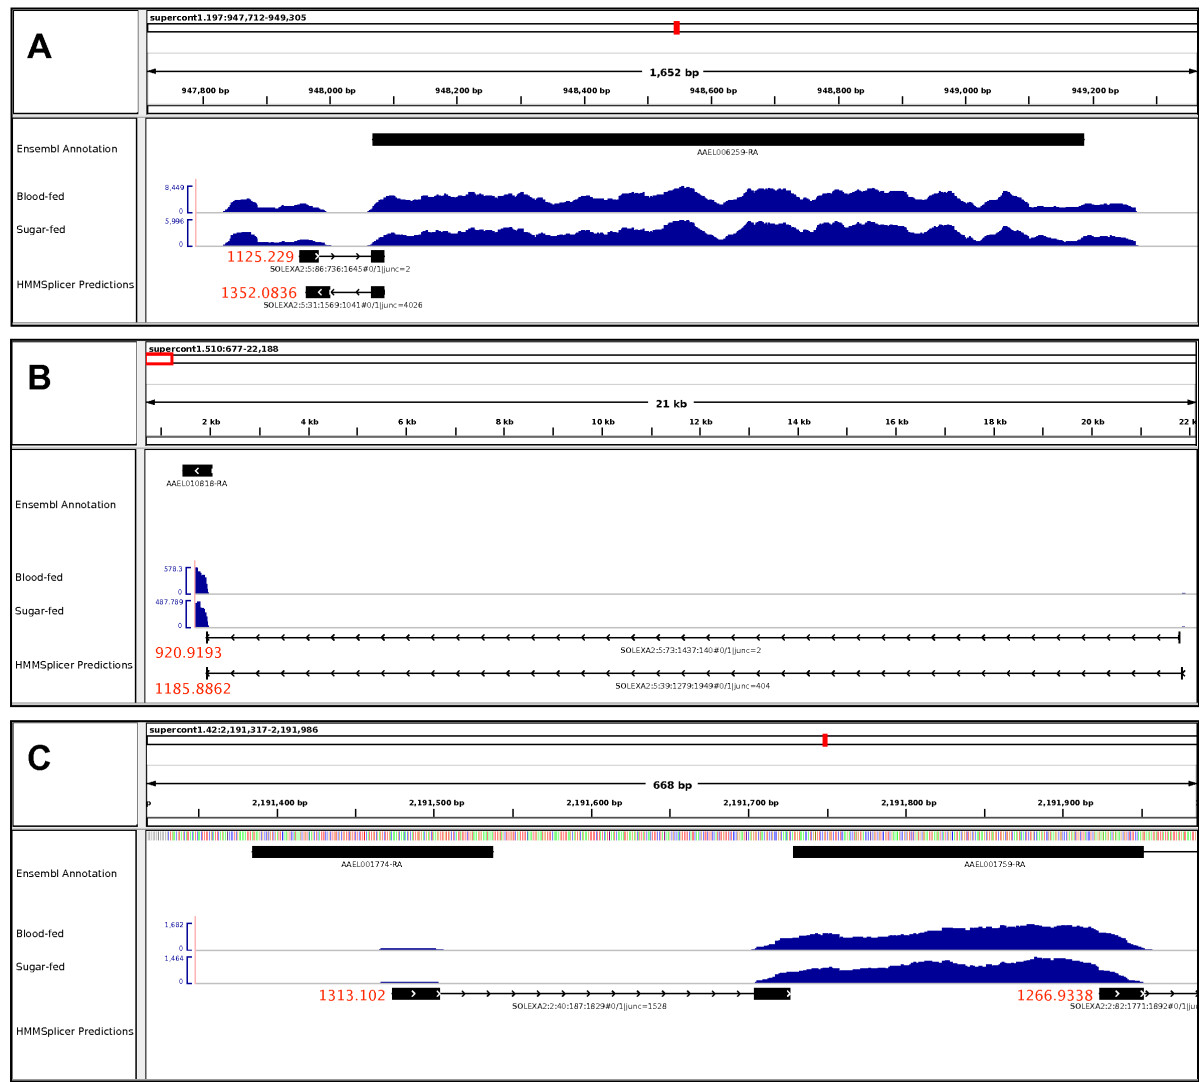
\includegraphics[width=.95\textwidth]{figures/figs/aedesHMMsplice.jpg}

\caption[Examples of amendments to the \Aa\ annotation supported by HMMSplicer results]{\sf \textbf{Examples of amendments to the \Aa\ annotation supported by HMMSplicer results:} Black bars in the top tracks represent the current gene annotations. Blue histograms in the second track represent the non-normalized coverage of RNA-seq reads at each position. The range of the histogram values shown in each view is depicted on the labeled y-axis of each RNA-seq track. Black boxes in the lower track represent splice-site predictions based on the RNA-seq reads using HMMSplicer determined in this study. Each function has a unique identifier listed below and its HMMSplicer score is listed in red. If multiple reads support a single junction, "junc = x" lists the number of supporting reads. This information provides evidence to link two islands of transcription as a single transcription event, therefore, exons of a common mRNA. All predicted junctions shown here also are supported by EST alignments. Genes are (A) AAEL006259; (B) AAEL010818; and (C) AAEL001774 and AAEL001759.

Excerpted from \cite{Bonizzoni2011}}
\label{fig:aedesHMMsplice}
\end{figure}

\begin{figure}[hp]
\centering
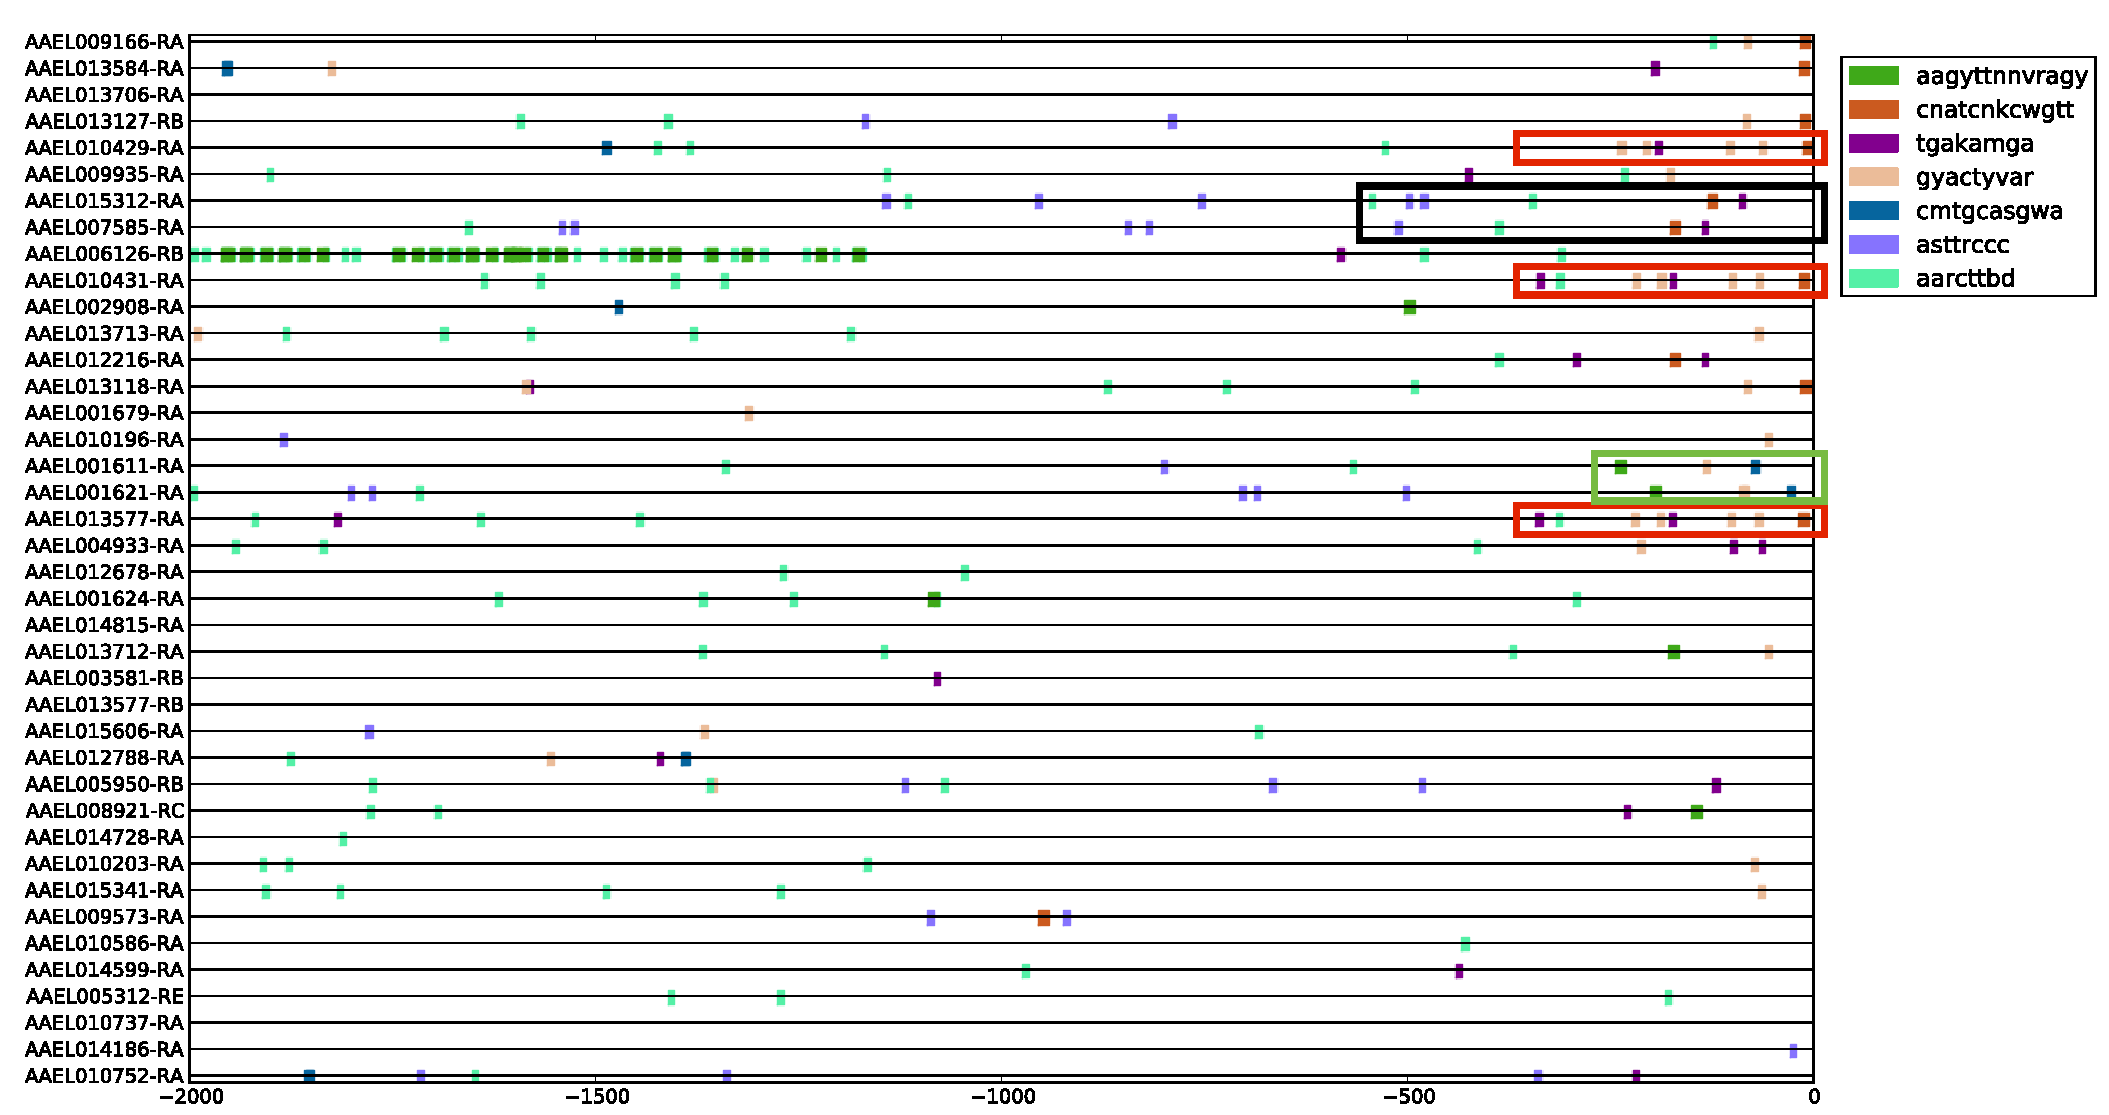
\includegraphics[width=.99\textwidth]{figures/figs/bonizzoni2011-cres.pdf}

\caption[Motif map of putative CREs from transcripts detected only in bloodfed female \Aa]{\sf \textbf{Motif map of putative CREs discovered by SCOPE using transcripts detected significantly only in bloodfed female \Aa:} Locations of representative SCOPE-derived CRE motifs in the 2000 bp upstream of the annotated translational start site in the 40 transcripts detected significantly only in bloodfed females. Transcript names on the left are ordered from most (top) to least (bottom) abundant.  Candidate CRMs are highlighted in like-colored rectangles.

Adapted from \cite{Bonizzoni2011}}
\label{fig:bonizzoni2011-cres}
\end{figure}
\begin{table}[hp]
 \begin{center} \sf
\begin{tabular}{cc}\toprule
\textbf{Distance from annotation (bp)} & \textbf{Predicted junctions}\\ \midrule
0-1000 & 1170\\
1001-2000 & 120\\
2001-4000 & 149\\
4001-8000 & 245\\
8001-16000 & 486\\
16001-32000 & 517\\
> 32000 & 854\\ \midrule
\textbf{Total} & \textbf{3541}\\ \bottomrule
 \end{tabular}
 \end{center}

\caption[Predicted novel junctions within various symmetric distance-windows from annotated transcripts]{\sf \textbf{Predicted novel junctions within various symmetric distance-windows from annotated transcripts:} \\
(Gene build AaegL1.2)\\
Excerpted from \cite{Bonizzoni2011}}

\label{tab:bonizzoni2011-novel-junx}
\end{table} 




\pagebreak
\section{Strain variation in the transcriptome of the dengue fever vector, \Aea}
\todo[inline]{import text for STRAIN VARIATION}
Figure \ref{fig:aa-diff-paralogs}

\begin{figure}[h]

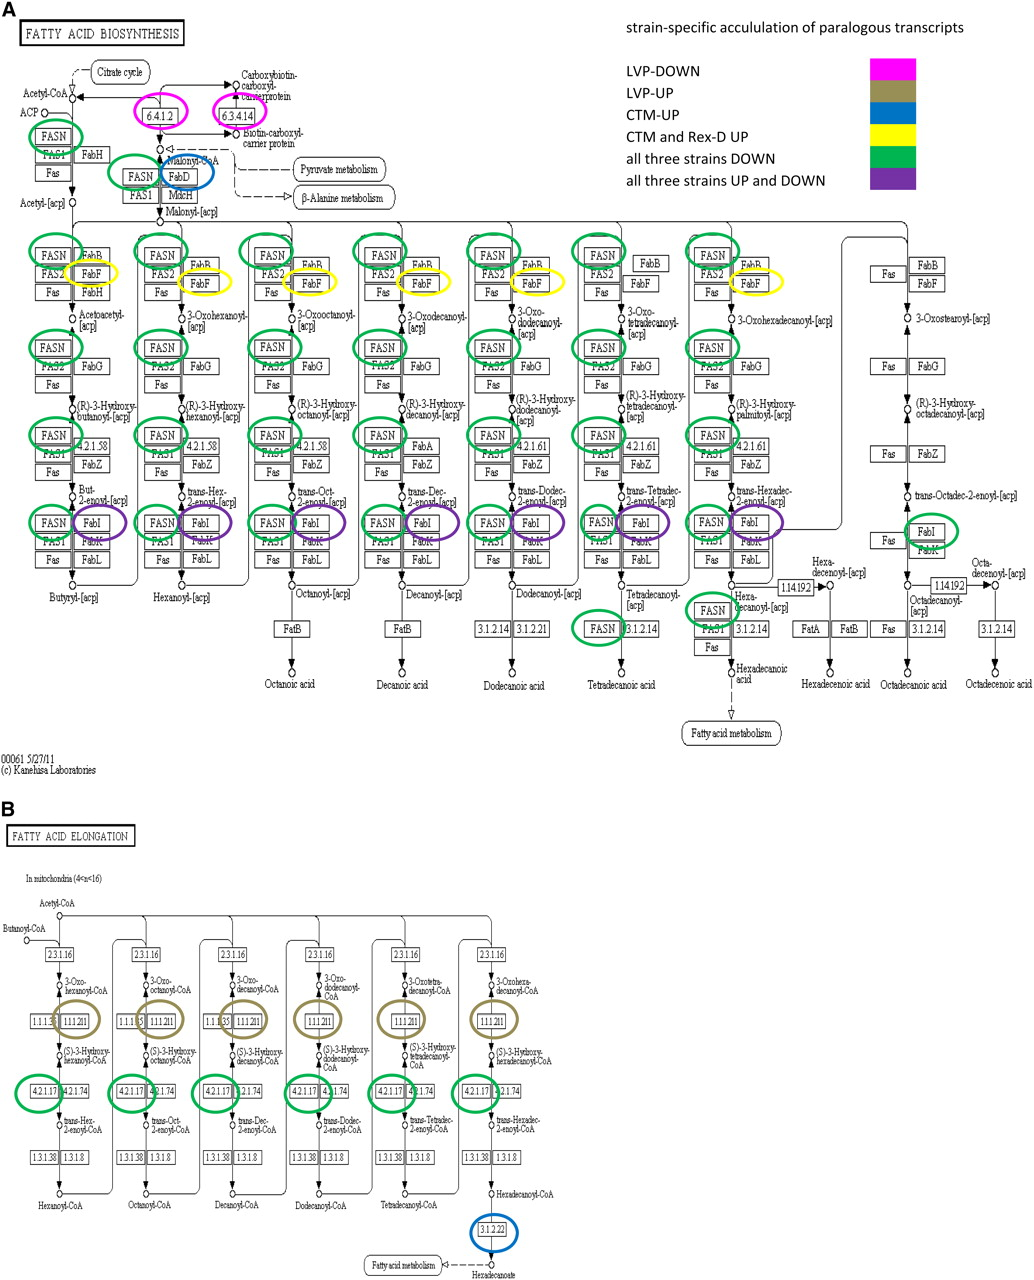
\includegraphics[width=.9\textwidth]{figures/figs/aa-diff-paralogs.jpg}

\caption[Fatty acid biosynthesis and elongation in mitochondria]{\sf \textbf{Fatty acid biosynthesis and elongation in mitochondria:} Proteins corresponding to transcripts accumulated in a strain-specific manner are circled in a color corresponding to the strain and condition defined in the legend (panels A and B).

Excerpted from \cite{bonizzoni2012strain}}
\label{fig:aa-diff-paralogs}
\end{figure}


\pagebreak
\section{Complex modulation of the \Aea transcriptome in response to dengue virus infection}
\todo[inline]{import text for COMPLEX MODULATION OF AEDES TXOME}
Figure \ref{fig:bonizzoni2012complex-cre}

\begin{figure}[hp]
\centering

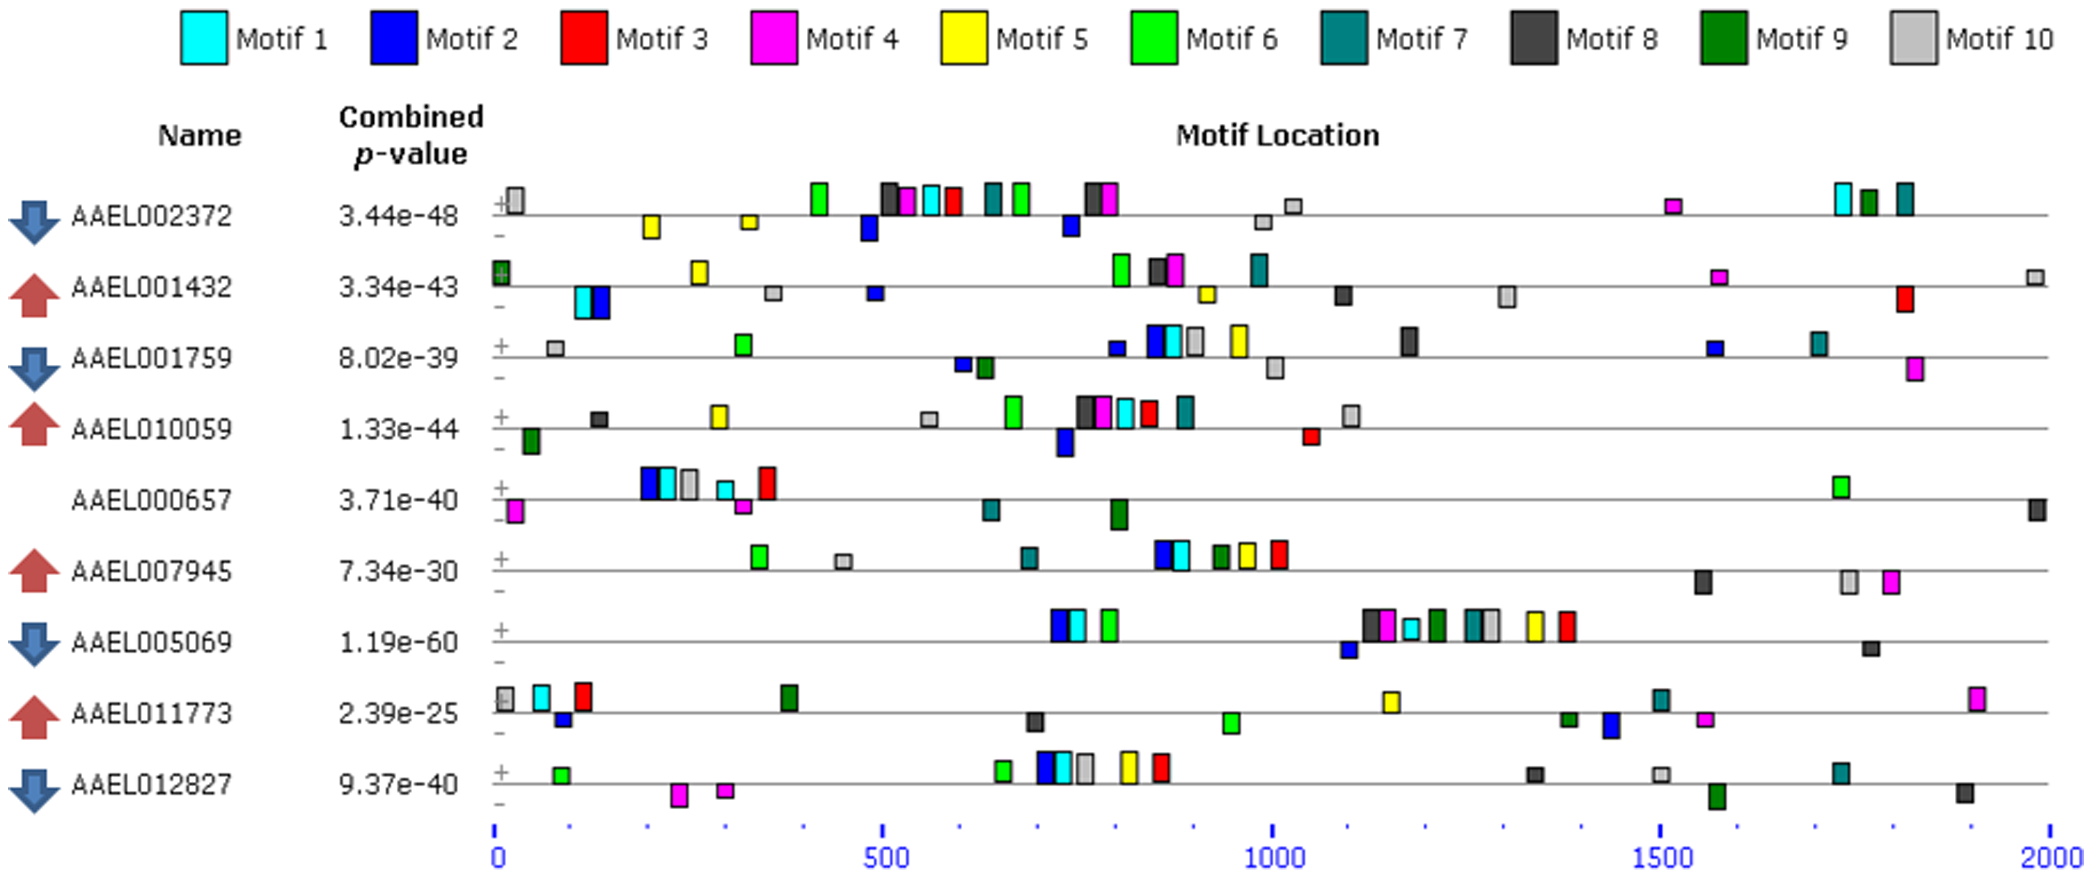
\includegraphics[width=.99\textwidth]{figures/figs/bonizzoni2012complex-cre.png}

\caption[MEME analysis of nine genes with \texorpdfstring{FPKM\textsubscript{DENVI}}{FPKM DENVI} ≥ 100 in carcasses and salivary glands at 14 dpi]{\sf \textbf{MEME analysis of nine genes with \texorpdfstring{FPKM\textsubscript{DENVI}}{FPKM DENVI} ≥ 100 in carcasses and salivary glands at 14 dpi} These genes also were identified with transcripts exhibiting significant differential accumulation in analyses of salivary gland samples of the Liverpool strain infected with DEV2 Thailand 16881 [26]. Colored boxes represent individual putative CREs and their locations in promoters of each gene. Red and blue arrows adjacent to Ensembl Gene ID indicate those genes whose transcripts were detected previously as more or less abundant following DENV infection [26]. Distances in base-pairs are provided below the schematic of each gene.
doi:10.1371/journal.pone.0050512.g004

Excerpted from \cite{bonizzoni2012complex}}
\label{fig:bonizzoni2012complex-cre}
\end{figure}

% \texorpdfstring{FPKM\textsubscript{DENVI}}{FPKM DENVI}




%%% Local Variables: ***
%%% mode: latex ***
%%% TeX-master: "thesis.tex" ***
%%% End: ***
